\documentclass[aspectratio=169, 11pt]{beamer}

\usepackage[spanish]{babel}
\usepackage[utf8]{inputenc}
\usepackage[T1]{fontenc}

\usetheme{Madrid}
\usecolortheme{default}

\definecolor{uncblue}{RGB}{0, 75, 135}
\definecolor{unclight}{RGB}{220, 235, 250}
\definecolor{uncaccent}{RGB}{200, 60, 50}
\definecolor{uncgray}{RGB}{100, 100, 100}
\definecolor{uncgreen}{RGB}{40, 140, 60}
\definecolor{uncyellow}{RGB}{255, 195, 0}

\setbeamercolor{structure}{fg=uncblue}
\setbeamercolor{palette primary}{bg=uncblue, fg=white}
\setbeamercolor{palette secondary}{bg=uncblue!80, fg=white}
\setbeamercolor{palette tertiary}{bg=uncblue!60, fg=white}
\setbeamercolor{frametitle}{bg=uncblue, fg=white}
\setbeamercolor{title}{fg=uncblue}
\setbeamercolor{block title}{bg=uncblue, fg=white}
\setbeamercolor{block body}{bg=unclight}
\setbeamercolor{block title alerted}{bg=uncaccent, fg=white}
\setbeamercolor{block body alerted}{bg=uncaccent!10}
\setbeamercolor{item}{fg=uncblue}

\setbeamerfont{title}{series=\bfseries, size=\Large}
\setbeamerfont{frametitle}{series=\bfseries}

\setbeamertemplate{navigation symbols}{}
\setbeamertemplate{footline}{%
  \hfill\insertframenumber/\inserttotalframenumber\hspace{4pt}\vspace{2pt}%
}

\usepackage{graphicx}
\graphicspath{{../}}
\usepackage{booktabs}
\usepackage{amsmath, amssymb}
\usepackage{tikz}
\usetikzlibrary{arrows.meta, positioning, decorations.pathreplacing}
\usepackage[table]{xcolor}
\usepackage{hyperref}

\newcommand{\highlight}[1]{\textcolor{uncaccent}{\textbf{#1}}}
\newcommand{\bref}[1]{\textcolor{uncgray}{\scriptsize [#1]}}

\newcommand{\objdone}{\textcolor{uncgreen}{\textbf{\checkmark}}}
\newcommand{\objpend}{\textcolor{gray!50}{$\circ$}}
\newcommand{\objnow}{\textcolor{uncyellow}{$\blacktriangleright$}}

\newcommand{\objectivetracker}[3]{%
  \vfill
  \centering
  \shorthandoff{>}
  \begin{tikzpicture}
    \node[fill=unclight, rounded corners=4pt, inner xsep=10pt, inner ysep=4pt] {%
      \footnotesize
      #1\;\textbf{Predicción de edad} \qquad
      #2\;\textbf{Sociodemográficos} \qquad
      #3\;\textbf{Biomarcador}%
    };
  \end{tikzpicture}
  \shorthandon{>}
}

\title{Estimación de la edad cerebral mediante autoencoders variacionales y aprendizaje multimodal a partir de conectividad funcional, datos estructurales y variables sociodemográficas}
\author{Nicolás Marcelo Bazán}
\institute{%
  Facultad de Matemática, Astronomía, Física y Computación\\
  Universidad Nacional de Córdoba\\[6pt]
  
\includegraphics[height=1cm]{00_tapa/figures/logo_famaf.png}
  \hspace{1cm}
  
\includegraphics[height=1cm]{00_tapa/figures/logo_unc.png}
}
\date{2026}

\begin{document}

\begin{frame}[plain]
  \vfill
  \centering
  {\usebeamerfont{title}\color{uncblue}\inserttitle\par}
  \vspace{0.35cm}
  {\usebeamerfont{subtitle}\color{black!80}\insertsubtitle\par}
  \vspace{0.55cm}
  {\usebeamerfont{author}\insertauthor\par}
  \vspace{0.2cm}
  {\usebeamerfont{institute}\insertinstitute\par}
  \vspace{0.35cm}
  {\usebeamerfont{date}\insertdate\par}
  \vfill
\end{frame}

\begin{frame}{Estructura de la presentación}
  \tableofcontents
\end{frame}


\section{Motivación}

\begin{frame}{El cerebro envejece}
  \begin{columns}[T]
    \begin{column}{0.55\textwidth}
      \begin{itemize}
        \item El cerebro cambia con la edad de forma gradual y predecible
        \item Se pierde volumen de \highlight{materia gris}, se adelgaza la corteza
        \item Cambian los patrones de \highlight{conectividad} entre regiones
        \item Enfermedades como el Alzheimer o la demencia frontotemporal \textbf{aceleran} este proceso
      \end{itemize}
    \end{column}
    \begin{column}{0.42\textwidth}
      \centering
      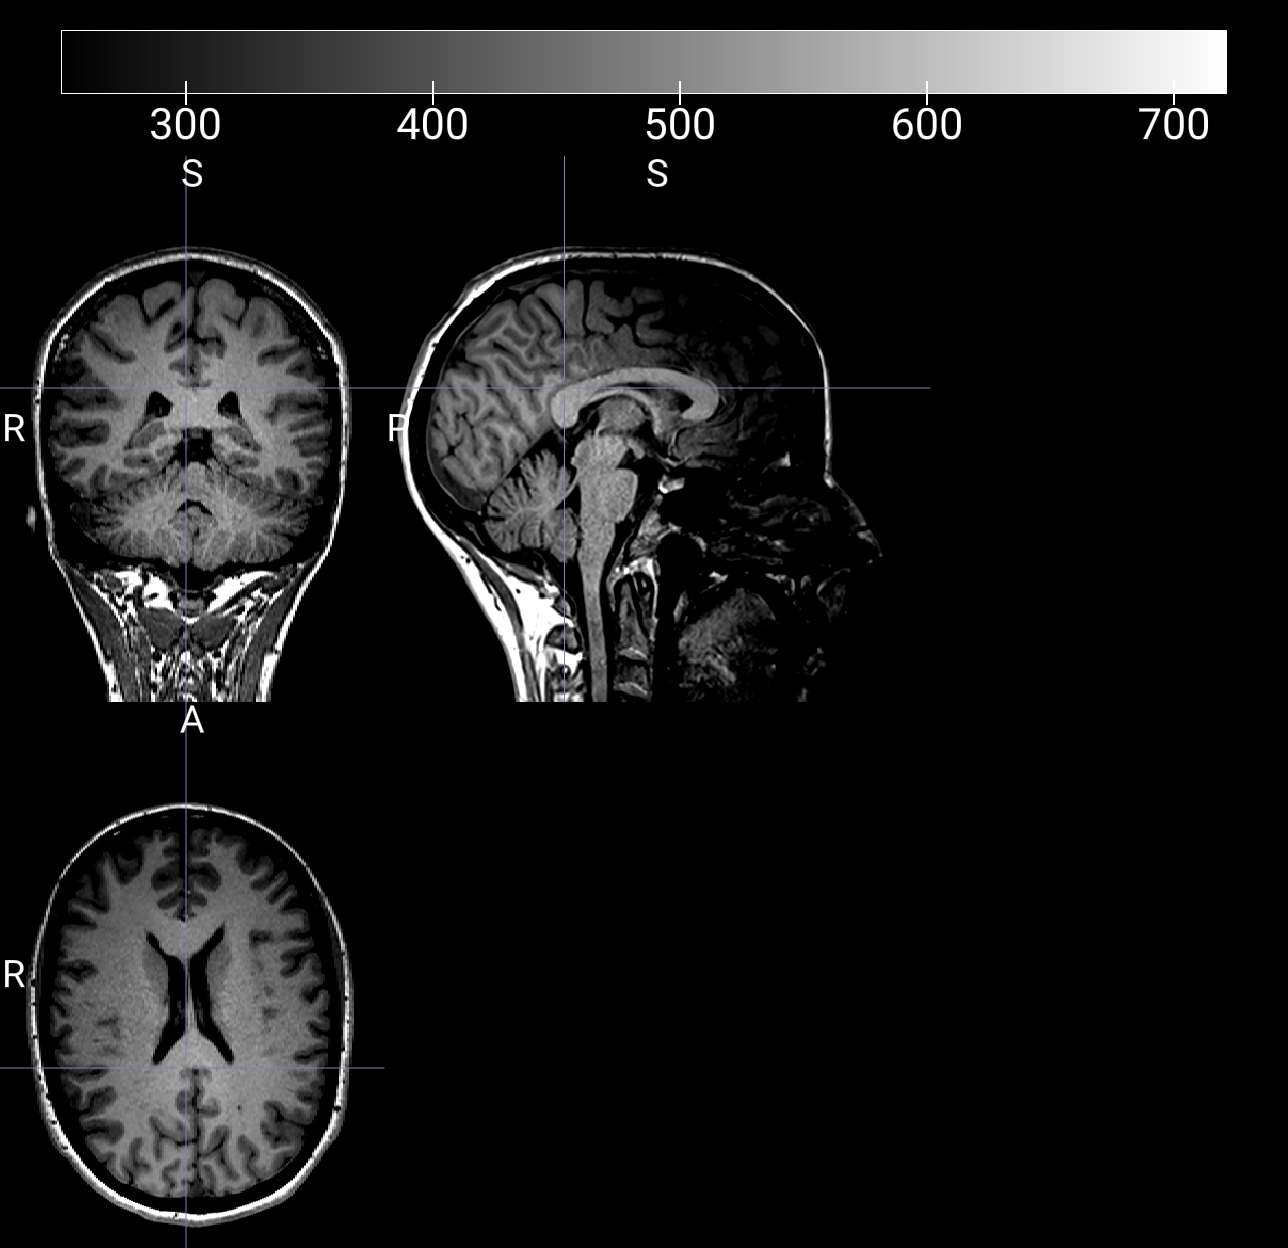
\includegraphics[width=\textwidth]{04_marco_teorico/images/t1_structural.png}\\[4pt]
      {\scriptsize Imagen T1w de resonancia magnética}
    \end{column}
  \end{columns}
\end{frame}

\begin{frame}{Brain Age Gap: la idea central}
  \centering
  \shorthandoff{>}
  \begin{tikzpicture}[
    box/.style={draw, rounded corners, text width=3cm, align=center,
                minimum height=1cm, font=\small},
    arr/.style={-{Stealth[length=3mm]}, thick, uncblue}
  ]
    \node[box, fill=unclight] (img) {Imagen cerebral\\del sujeto};
    \node[box, fill=unclight, right=1.8cm of img] (model) {Modelo\\predictivo};
    \node[box, fill=unclight, right=1.8cm of model] (pred) {Edad predicha\\$\hat{y} = 72$ años};
    \draw[arr] (img) -- (model);
    \draw[arr] (model) -- (pred);
  \end{tikzpicture}
  \shorthandon{>}

  \vspace{0.3cm}
  \begin{columns}[T]
    \begin{column}{0.46\textwidth}
      \begin{block}{Si la edad real es 65}
        \centering
        Gap $= 72 - 65 = \highlight{+7}$\\[3pt]
        {\small Envejecimiento \textbf{acelerado}}
      \end{block}
    \end{column}
    \begin{column}{0.46\textwidth}
      \begin{block}{Si la edad real es 78}
        \centering
        Gap $= 72 - 78 = \textcolor{uncgreen}{\textbf{-6}}$\\[3pt]
        {\small Cerebro ``más joven''}
      \end{block}
    \end{column}
  \end{columns}

  \vspace{0.25cm}
  {\small \textbf{Objetivos de este trabajo:}
  \begin{enumerate}
    \item \textbf{Obj.\ 1:} Predecir la edad cerebral combinando múltiples fuentes de neuroimagen
    \item \textbf{Obj.\ 2:} Analizar cómo variables sociodemográficas modulan la predicción
    \item \textbf{Obj.\ 3:} Explorar la viabilidad como biomarcador de envejecimiento acelerado
  \end{enumerate}
  }
\end{frame}


\section{Datos y contexto}

\begin{frame}[shrink=5]{Los datos de neuroimagen}
  \begin{columns}[T]
    \begin{column}{0.52\textwidth}
      {\small \textbf{Datos estructurales (T1w):}}
      \vspace{-0.1cm}
      \begin{itemize}\setlength{\itemsep}{1pt}
        \item \highlight{MRI}: técnica no invasiva; imágenes \textbf{T1w} distinguen materia gris, blanca y LCR
        \item \highlight{Materia gris}: cuerpos neuronales; volumen \textbf{disminuye con la edad}
        \item Atlas \highlight{AAL}: \textbf{116 regiones} anatómicas (espacio estándar MNI152)
      \end{itemize}

      \vspace{0.05cm}
      {\small \textbf{Datos funcionales (fMRI):}}
      \vspace{-0.1cm}
      \begin{itemize}\setlength{\itemsep}{1pt}
        \item \highlight{fMRI} en reposo: actividad cerebral indirecta (señal BOLD)
        \item Serie temporal por región; regiones sincronizadas $\rightarrow$ \textbf{funcionalmente conectadas}
      \end{itemize}

      \vspace{0.02cm}
      {\footnotesize \textbf{En este trabajo:} 116 volúmenes de materia gris + matrices de conectividad funcional por sujeto.}
    \end{column}
    \begin{column}{0.45\textwidth}
      \centering
      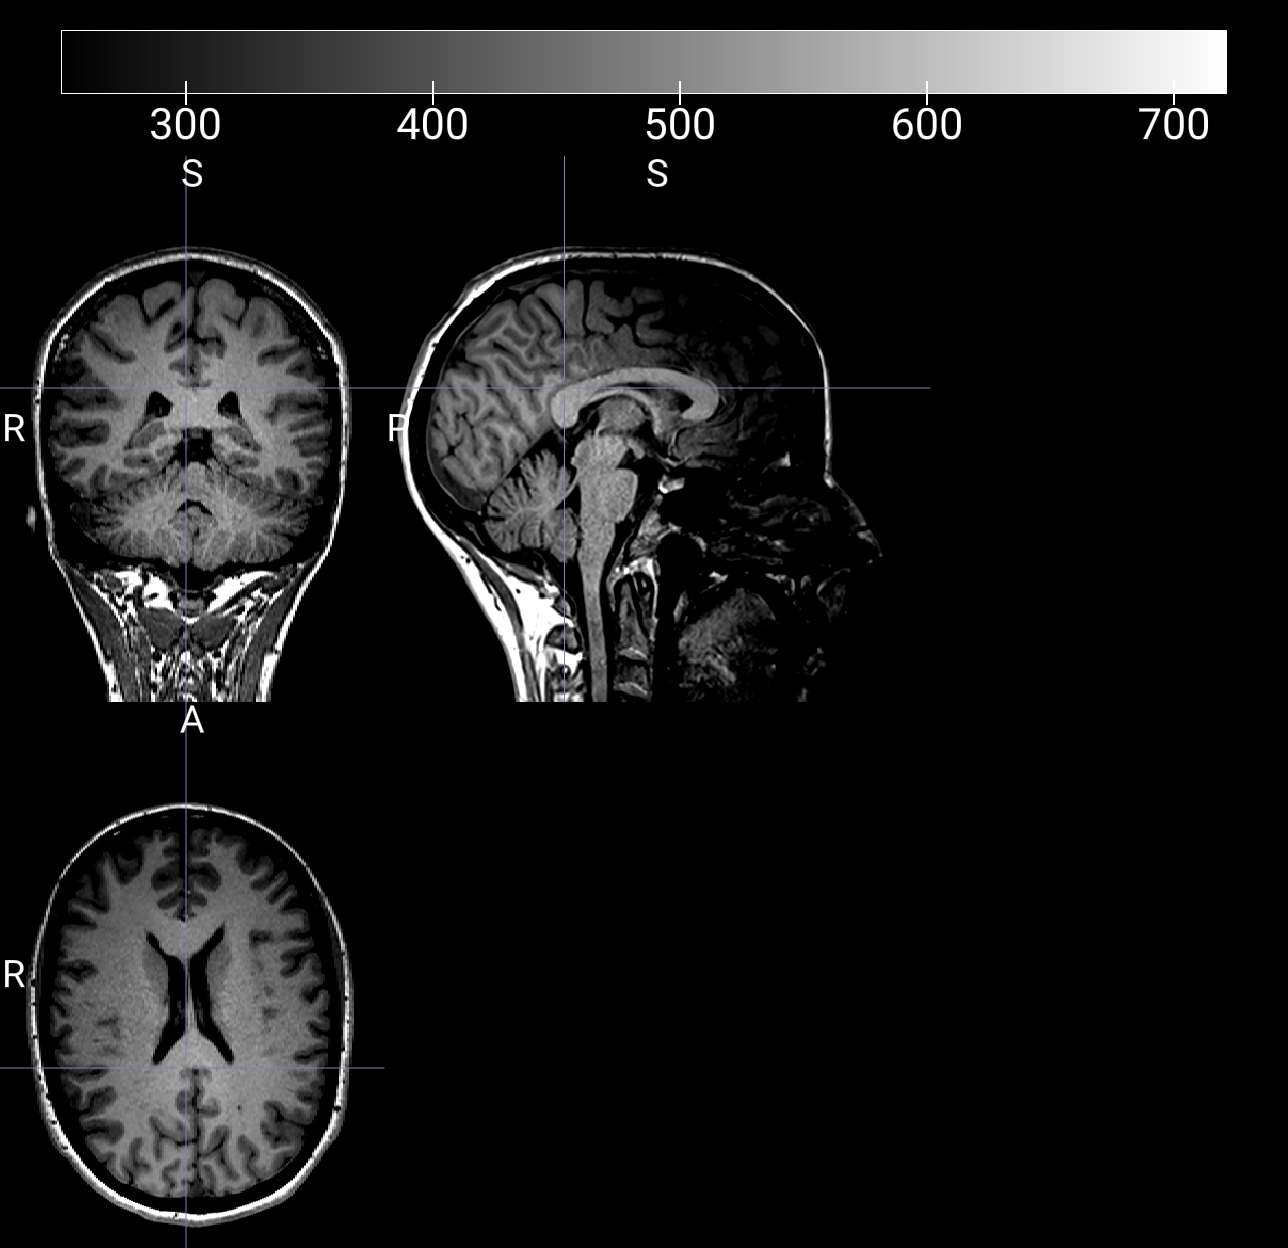
\includegraphics[width=0.52\textwidth]{04_marco_teorico/images/t1_structural.png}\\[1pt]
      {\scriptsize Imagen T1w}\\[3pt]
      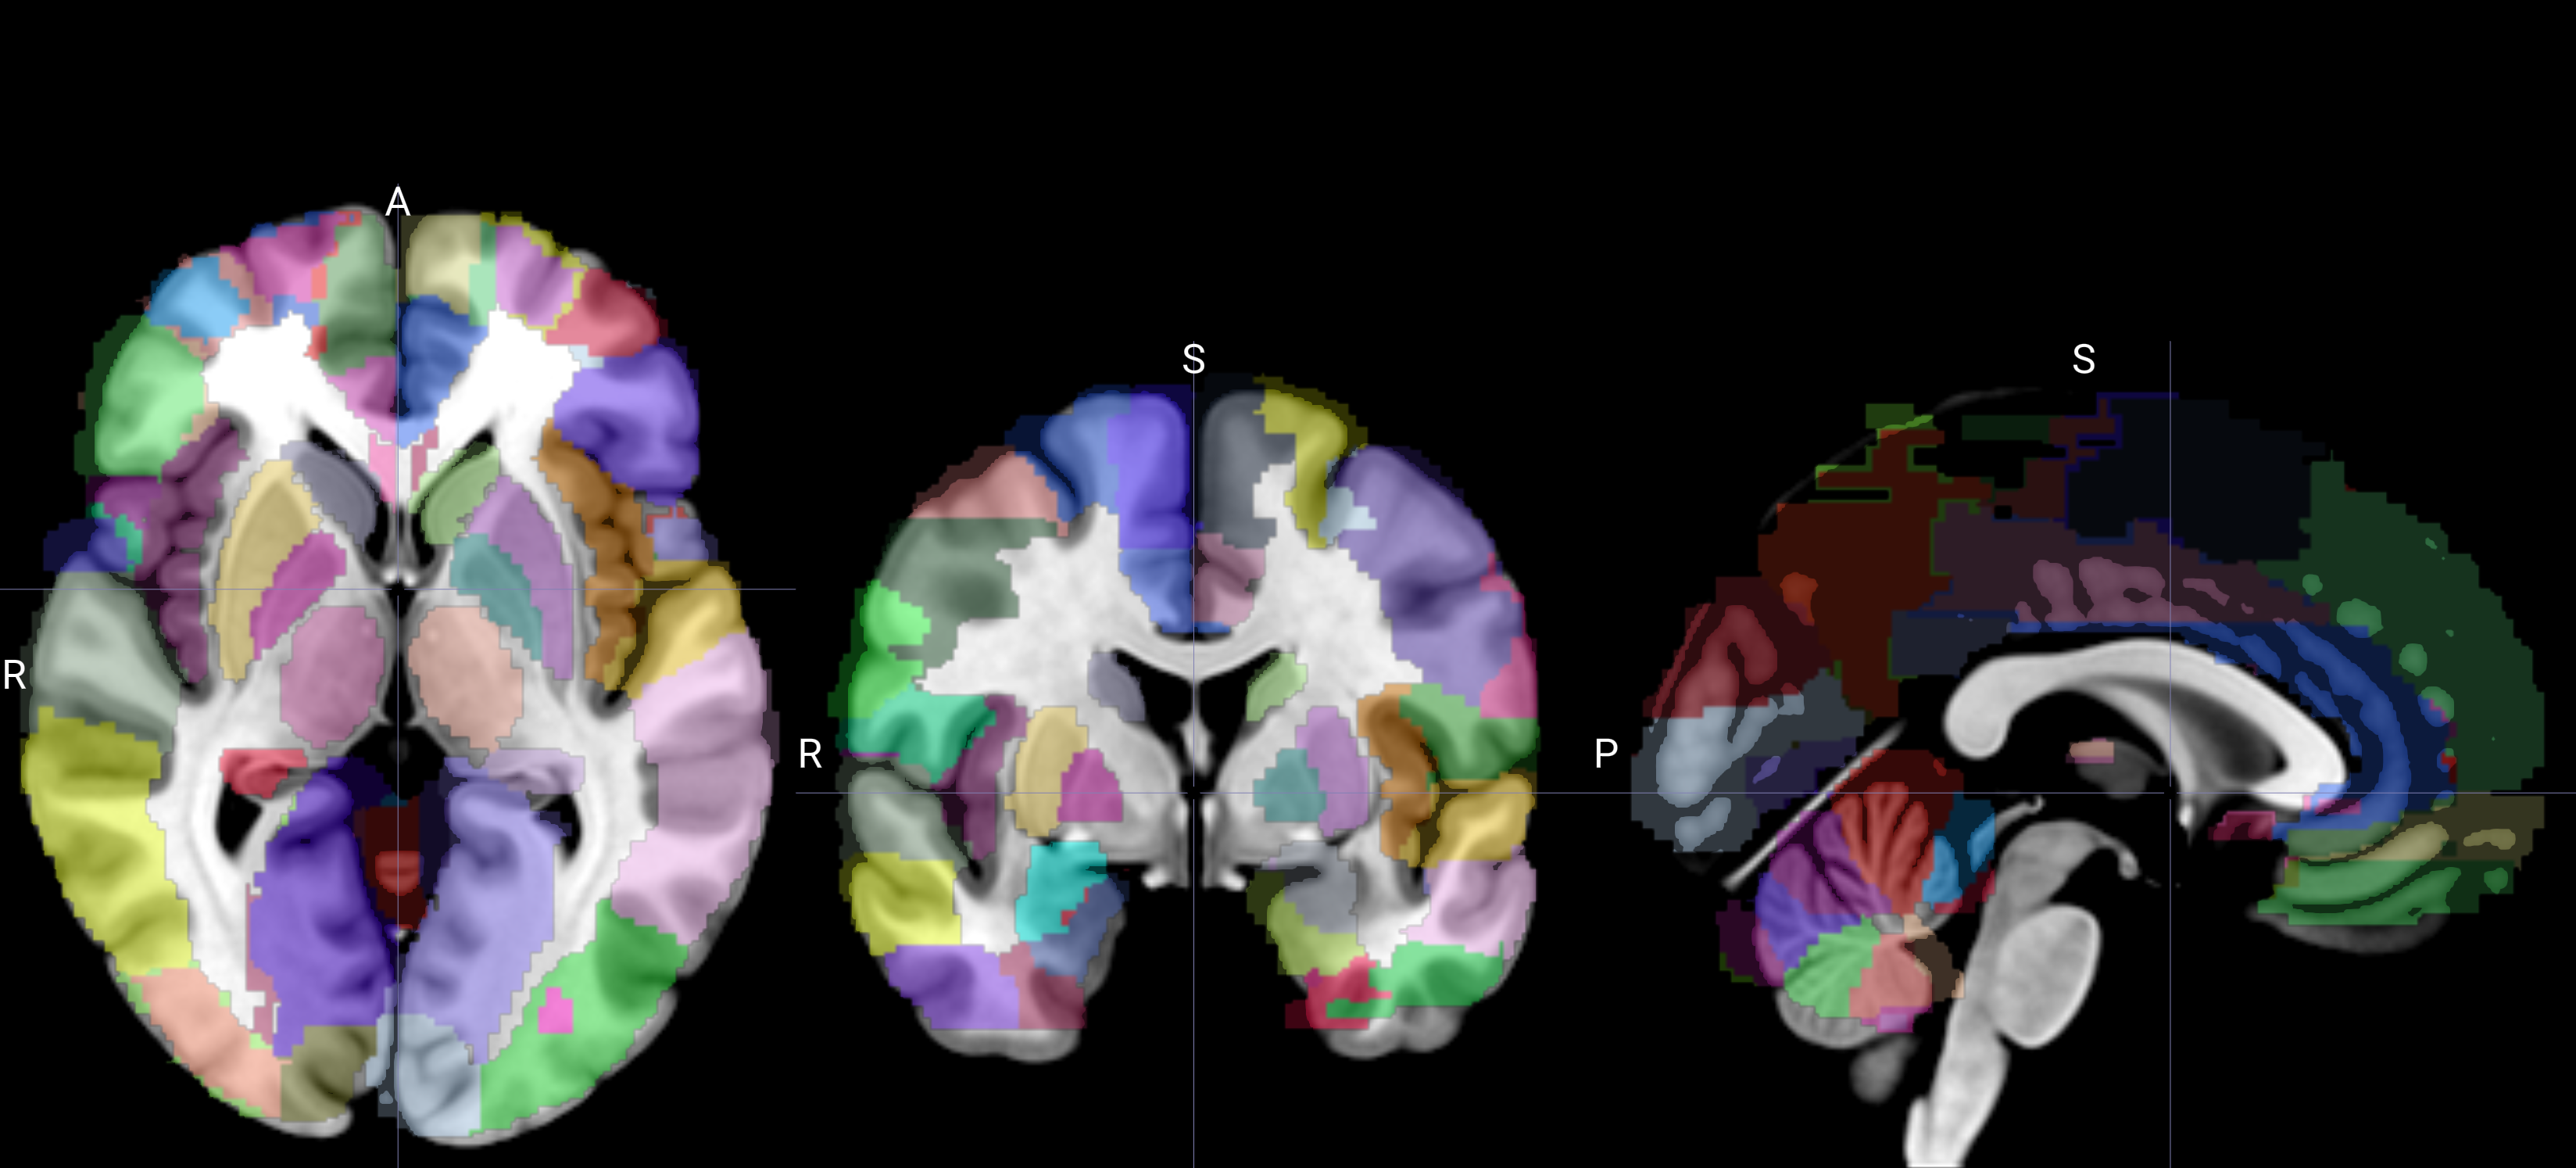
\includegraphics[width=0.52\textwidth]{04_marco_teorico/images/mni152+atlas.png}\\[1pt]
      {\scriptsize Atlas AAL: 116 regiones}
    \end{column}
  \end{columns}
\end{frame}

\begin{frame}[shrink=5]{Conectividad funcional}
  \centering
  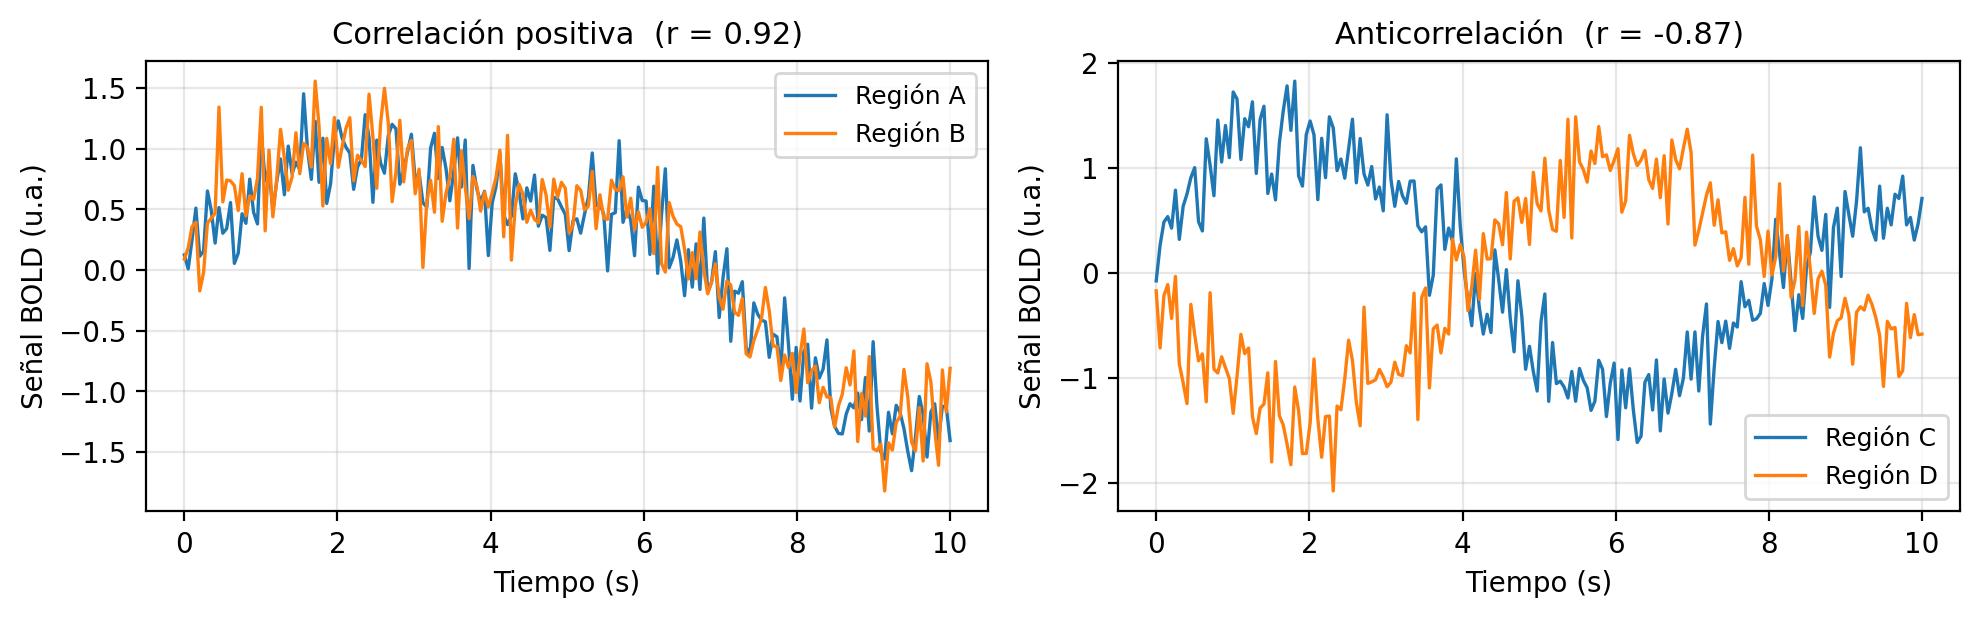
\includegraphics[width=0.75\textwidth]{04_marco_teorico/images/timeseries_correlation.png}

  \vspace{0.1cm}
  \begin{columns}[c]
    \begin{column}{0.48\textwidth}
      \begin{itemize}
        \item Se calcula la \highlight{correlación de Pearson} entre cada par de regiones
        \item Resultado: matriz simétrica $116 \times 116$
        \item Triángulo superior: \highlight{6670 valores} por sujeto
      \end{itemize}
    \end{column}
    \hspace{-0.8cm}
    \begin{column}{0.35\textwidth}
      \centering
      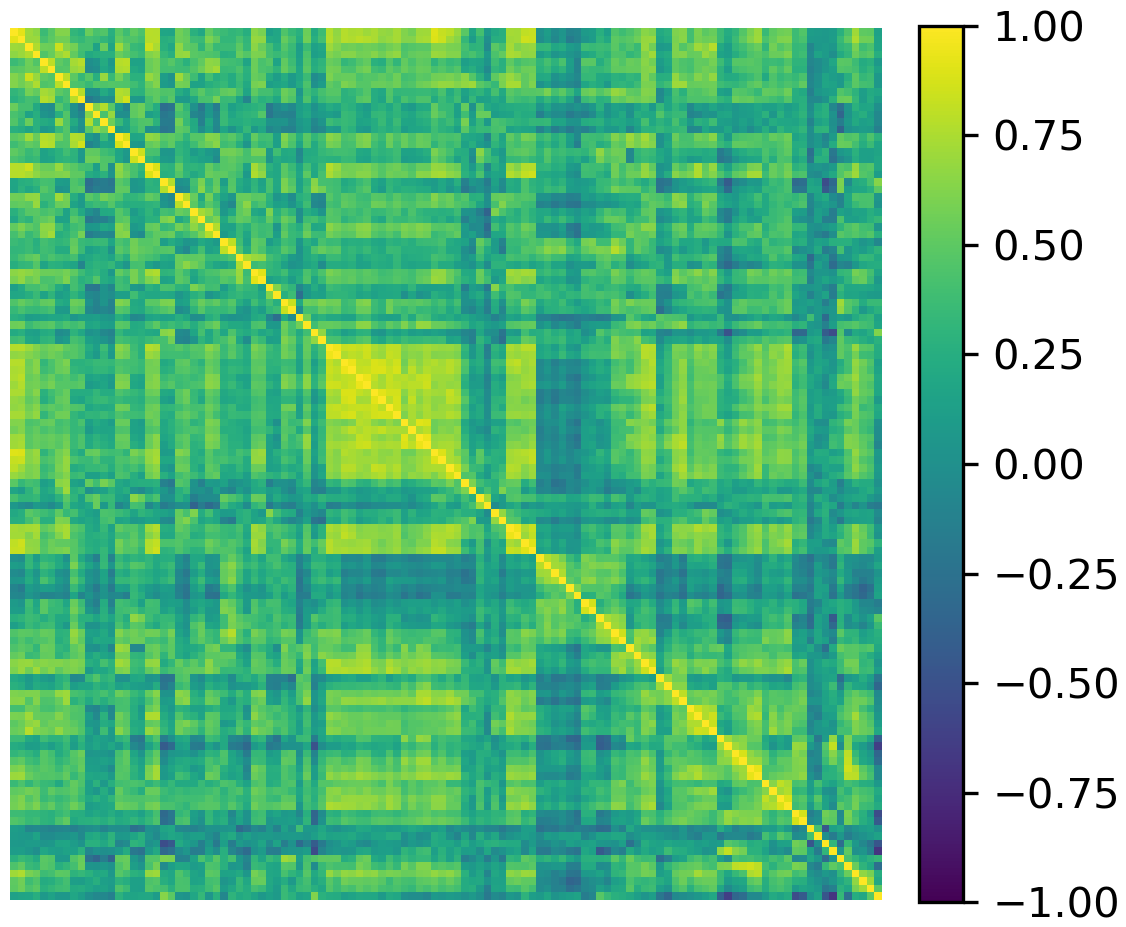
\includegraphics[width=0.80\textwidth]{04_marco_teorico/images/fc_example.png}\\[-4pt]
      {\scriptsize Matriz FC $116 \times 116$}
    \end{column}
  \end{columns}
\end{frame}

\begin{frame}{La cohorte: RedLaT}
  \begin{columns}[T]
    \begin{column}{0.52\textwidth}
      {\small \textbf{Red Latinoamericana de Neurodegeneración:} datos clínicos y de neuroimagen de múltiples centros de América Latina. Heterogeneidad socioeconómica, cultural y de protocolos.}

      \vspace{0.1cm}
      {\small \textbf{Datos integrados:} matrices FC, volúmenes T1w, metadatos clínicos, variables demográficas ($\sim$75\%).}

      \vspace{1.2cm}
      \centering
      \shorthandoff{>}
      \begin{tikzpicture}[scale=0.92, transform shape,
        box/.style={draw, rounded corners, align=center, text width=1.5cm,
                    minimum height=0.55cm, font=\footnotesize},
        arr/.style={-{Stealth[length=2.5mm]}, thick, uncblue}
      ]
        \node[box, fill=unclight] (fc) {FC\\$N{=}1365$};
        \node[box, fill=unclight, right=0.3cm of fc] (meta) {Meta\\$N{=}1327$};
        \node[box, fill=unclight, right=0.3cm of meta] (t1) {T1w\\$N{=}2748$};
        \node[box, fill=uncaccent!15, right=0.3cm of t1, text width=1.7cm] (final)
          {\textbf{Final}\\$\boldsymbol{N{=}1245}$};
        \draw[arr] (fc) -- (meta);
        \draw[arr] (meta) -- (t1);
        \draw[arr] (t1) -- (final);
      \end{tikzpicture}
      \shorthandon{>}
    \end{column}
    \begin{column}{0.45\textwidth}
      \centering
      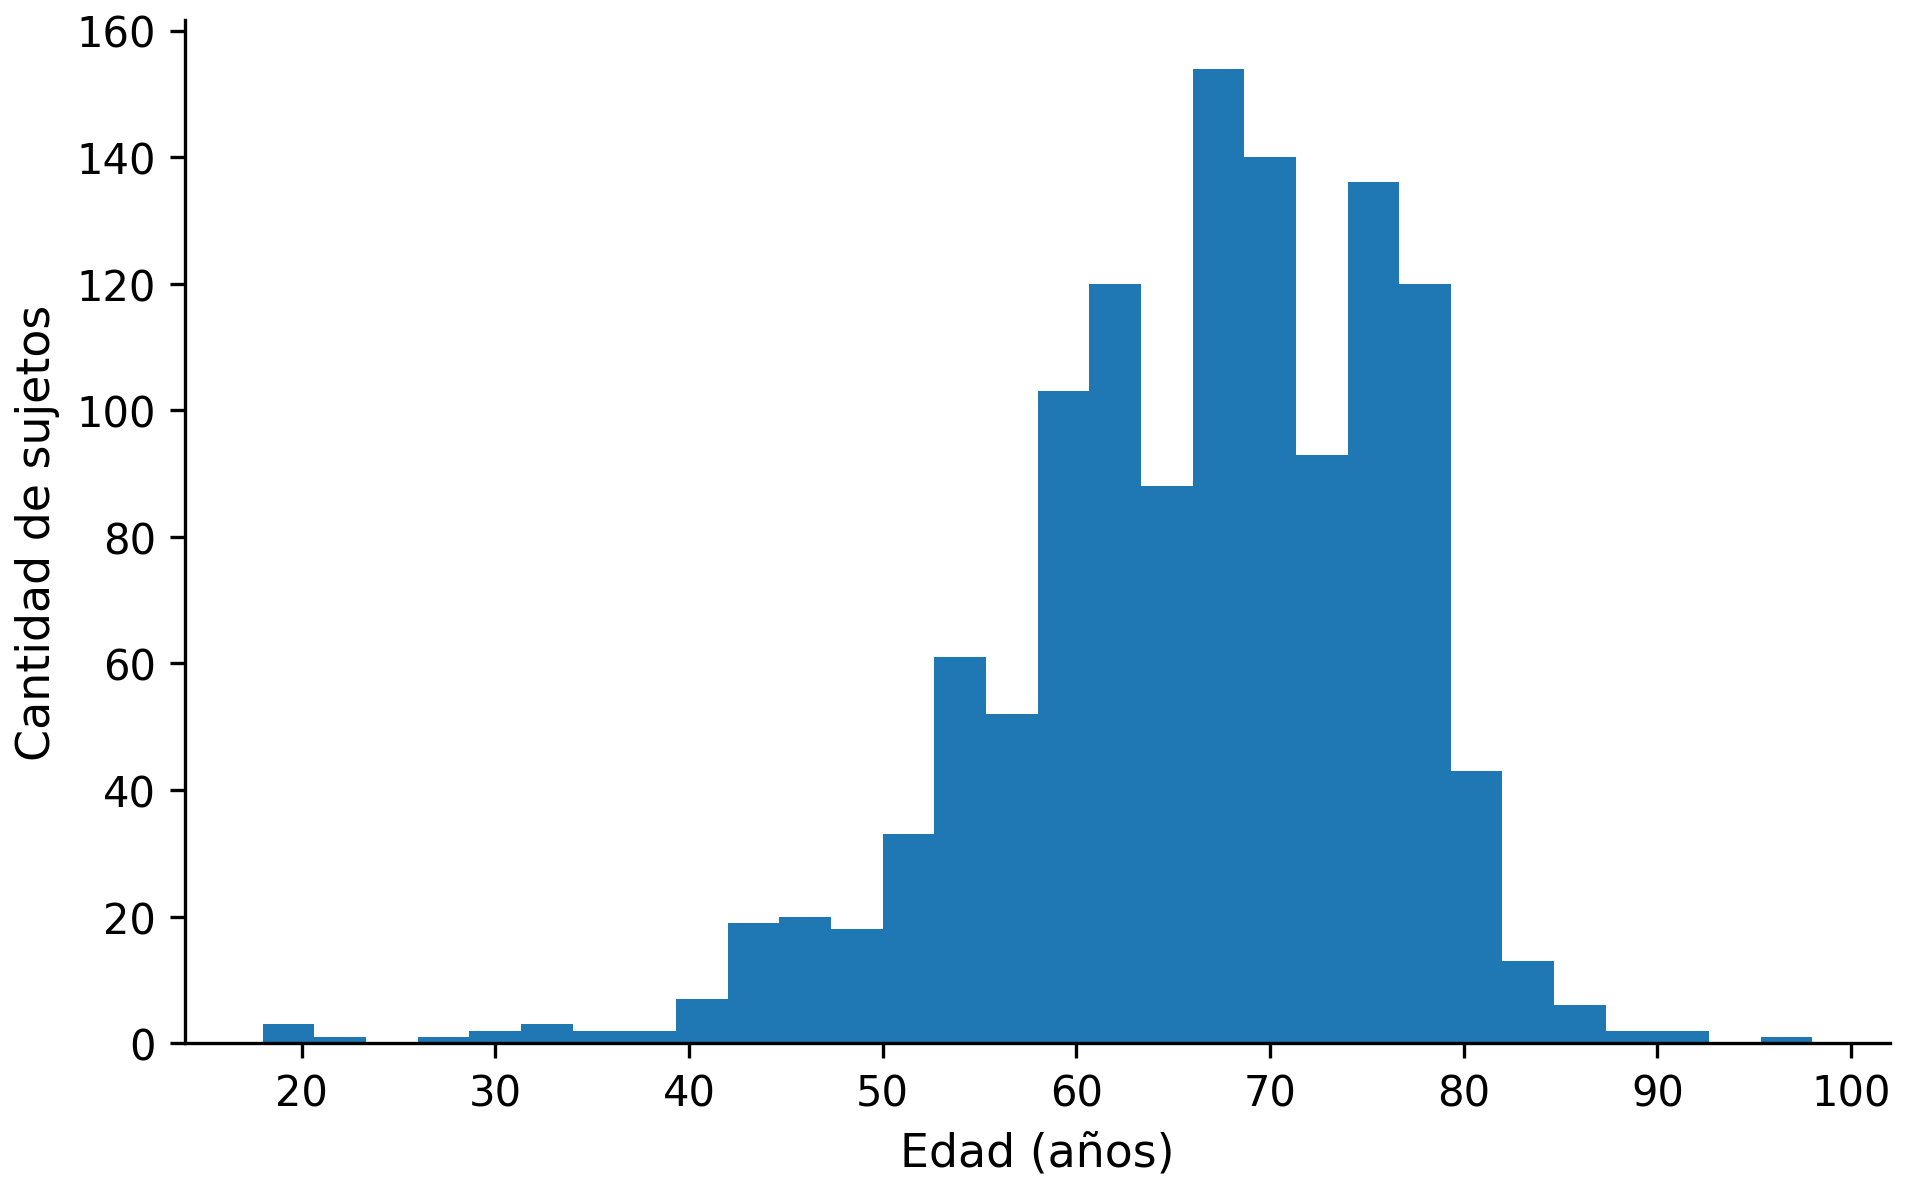
\includegraphics[width=0.95\textwidth]{05_datos_cohorte/images/age_hist.png}\\[2pt]
      {\scriptsize Distribución de edades (rango 18--98)}

      \vspace{0.15cm}
      {\small
      \begin{tabular}{lrrr}
        \toprule
        & \textbf{CN} & \textbf{AD} & \textbf{FTD} \\
        \midrule
        $N$ & 526 & 422 & 297 \\
        Edad & $64 \pm 15$ & $72 \pm 10$ & $66 \pm 10$ \\
        \bottomrule
      \end{tabular}}
    \end{column}
  \end{columns}
\end{frame}


\section{Métodos y pipeline}

\begin{frame}{El desafío: alta dimensionalidad}
  \begin{alertblock}{Problema ``small-n, large-p''}
    \highlight{6670} features de conectividad funcional, pero solo $N = \highlight{1245}$ sujetos $\rightarrow$ alto riesgo de \textbf{sobreajuste}.
  \end{alertblock}

  \vspace{0.3cm}
  \begin{columns}[T]
    \begin{column}{0.48\textwidth}
      \begin{block}{¿Por qué no usar FC directamente?}
        {\small
        \begin{itemize}\setlength{\itemsep}{3pt}
          \item La FC \textit{promediada globalmente} no correlaciona con la edad ($r \approx 0$)
          \item La información útil está en \highlight{patrones específicos} entre regiones
          \item Al promediar, las señales opuestas se cancelan
        \end{itemize}}
      \end{block}
    \end{column}
    \begin{column}{0.48\textwidth}
      \begin{block}{Solución}
        {\small
        \begin{itemize}\setlength{\itemsep}{3pt}
          \item \textbf{Reducción de dimensionalidad} para capturar patrones relevantes
          \item De \highlight{6670} a \highlight{64} dimensiones
          \item Preservar estructura, eliminar ruido
        \end{itemize}}
      \end{block}
    \end{column}
  \end{columns}
\end{frame}

\begin{frame}[shrink=10]{$\beta$-VAE: compresión inteligente de la conectividad}
  \begin{columns}[T]
    \begin{column}{0.50\textwidth}
      {\small \textbf{Autoencoder:} red que comprime y reconstruye. El ``cuello de botella'' retiene solo lo esencial.}

      \vspace{0.08cm}
      {\small \textbf{VAE --- la diferencia clave:}
      cada entrada no es un \textbf{punto} sino una \highlight{distribución} ($\mu$, $\sigma$).
      Truco de reparametrización:}
      \vspace{-0.15cm}
      \[
        z = \mu + \sigma \odot \epsilon, \quad \epsilon \sim \mathcal{N}(0, I)
      \]

      \vspace{-0.25cm}
      {\small Cada vez que se ``corre'', el resultado puede ser distinto (naturaleza probabilística).}

      \vspace{0.05cm}
      {\small \textbf{$\beta$-VAE:} $\mathcal{L} = \mathcal{L}_{\text{rec}} + \beta \cdot D_{KL}$.\;
      $\beta$ pondera reconstrucción vs.\ regularización; $\beta \to 0$ \highlight{recupera el AE clásico}.\\
      Optuna: $\beta = 0{,}057 \ll 1$ $\rightarrow$ comportamiento cercano a AE para esta tarea.}

      \vspace{0.15cm}
      {\small \textbf{En este trabajo:} $6670 \to 64$ dimensiones (99\% de compresión). Para la predicción se usa $\mu$ directamente (determinístico). El espacio latente regularizado produce representaciones más robustas para la tarea de predicción de edad.}
    \end{column}
    \begin{column}{0.48\textwidth}
      {\scriptsize \textbf{AE clásico} --- cada entrada $\to$ \textbf{punto fijo} $z$:}
      \vspace{0.05cm}
      \centering
      \shorthandoff{>}
      \begin{tikzpicture}[scale=0.85, transform shape,
        >=Stealth,
        neuron/.style={circle, draw, thick, minimum size=0.45cm, inner sep=0pt},
        input/.style={neuron, fill=teal!20},
        hidden/.style={neuron, fill=blue!15},
        lat/.style={neuron, fill=orange!25},
        conn/.style={-, gray!50, thin},
        arr/.style={->, thick},
      ]
        \foreach \i in {1,...,4} {
          \node[input] (in\i) at (0, -\i*0.9 + 2.25) {};
        }
        \node[above=0.1cm of in1, font=\small\bfseries] {$\mathbf{x}$};
        \foreach \i in {1,...,3} {
          \node[hidden] (h1\i) at (2.2, -\i*0.9 + 1.8) {};
        }
        \foreach \i in {1,...,2} {
          \node[lat] (z\i) at (4.4, -\i*0.9 + 1.35) {};
        }
        \node[above=0.1cm of z1, font=\small\bfseries] {$\mathbf{z}$};
        \foreach \i in {1,...,3} {
          \node[hidden] (h2\i) at (6.6, -\i*0.9 + 1.8) {};
        }
        \foreach \i in {1,...,4} {
          \node[input] (out\i) at (8.8, -\i*0.9 + 2.25) {};
        }
        \node[above=0.1cm of out1, font=\small\bfseries] {$\tilde{\mathbf{x}}$};
        \foreach \i in {1,...,4} { \foreach \j in {1,...,3} { \draw[conn] (in\i) -- (h1\j); } }
        \foreach \i in {1,...,3} { \foreach \j in {1,...,2} { \draw[conn] (h1\i) -- (z\j); } }
        \foreach \i in {1,...,2} { \foreach \j in {1,...,3} { \draw[conn] (z\i) -- (h2\j); } }
        \foreach \i in {1,...,3} { \foreach \j in {1,...,4} { \draw[conn] (h2\i) -- (out\j); } }
        \node[font=\scriptsize, gray] at (1.1, -2.2) {Encoder};
        \node[font=\scriptsize, gray] at (7.7, -2.2) {Decoder};
        \node[font=\tiny, gray, below=0.15cm of z2] {punto fijo};
      \end{tikzpicture}
      \shorthandon{>}

      \vspace{0.15cm}
      {\scriptsize \textbf{VAE} --- cada entrada $\to$ \textbf{distribución} $(\mu, \sigma)$:}
      \vspace{0.05cm}
      \centering
      \shorthandoff{>}
      \begin{tikzpicture}[scale=0.82, transform shape,
        >=Stealth,
        encblock/.style={draw, thick, rounded corners=3pt, minimum height=0.8cm,
                      minimum width=1.3cm, fill=blue!12, font=\small, align=center},
        decblock/.style={draw, thick, rounded corners=3pt, minimum height=0.8cm,
                      minimum width=1.3cm, fill=red!12, font=\small, align=center},
        arr/.style={->, thick},
      ]
        \node (x) {$x$};
        \node[encblock, right=0.5cm of x] (enc) {Encoder\\[-2pt]{\tiny $q(z \mid x)$}};
        \node[draw, thick, circle, minimum size=0.7cm, fill=yellow!15, font=\small, above right=0.5cm and 1cm of enc] (mu) {$\mu$};
        \node[draw, thick, circle, minimum size=0.7cm, fill=orange!15, font=\small, below right=0.5cm and 1cm of enc] (sigma) {$\sigma$};
        \node[draw, thick, circle, minimum size=0.7cm, fill=green!15, font=\small, right=2.8cm of enc] (z) {$z$};
        \node[decblock, right=0.8cm of z] (dec) {Decoder\\[-2pt]{\tiny $p(x \mid z)$}};
        \node[right=0.5cm of dec] (xhat) {$\tilde{x}$};

        \node[below=0.5cm of z, font=\tiny] (eps) {$\epsilon \sim \mathcal{N}(0, I)$};

        \draw[arr] (x) -- (enc);
        \draw[arr] (enc) |- (mu);
        \draw[arr] (enc) |- (sigma);
        \draw[arr] (mu) -- (z);
        \draw[arr] (sigma) -- (z);
        \draw[arr, dashed] (eps) -- (z);
        \draw[arr] (z) -- (dec);
        \draw[arr] (dec) -- (xhat);

        \node[above=0.05cm of z, font=\tiny\itshape] {$z = \mu + \sigma \odot \epsilon$};
      \end{tikzpicture}
      \shorthandon{>}

    \end{column}
  \end{columns}
\end{frame}

\begin{frame}[shrink=3]{Pipeline completo}
  \centering
  \shorthandoff{>}
  \begin{tikzpicture}[scale=0.68, transform shape,
    node distance=0.5cm and 0.8cm,
    block/.style={rectangle, draw, rounded corners, text width=2.6cm,
                  minimum height=0.65cm, align=center, font=\small},
    data/.style={rectangle, draw, dashed, rounded corners, text width=2.4cm,
                 minimum height=0.55cm, align=center, font=\small, fill=gray!10},
    arrow/.style={-{Stealth[length=2.5mm]}, thick, uncblue}
  ]
    \node[data] (fc) {Matrices FC\\$(116 \times 116)$};
    \node[data, right=2.2cm of fc] (t1w) {Volúmenes T1w\\(116 regiones)};

    \node[block, below=of fc, fill=unclight] (preproc) {Fisher $z$ + vectorización\\(6670 dims)};
    \node[block, below=of preproc, fill=unclight] (vae) {$\beta$-VAE Encoder};
    \node[data, below=of vae] (emb) {Embeddings $\mu$ (64 dims)};
    \node[block, below=0.6cm of emb, xshift=1.1cm, fill=uncaccent!15] (concat) {Concatenación (180 dims)};
    \node[block, below=of concat, fill=unclight] (xgb) {XGBoost};
    \node[data, below=of xgb] (pred) {Edad predicha $\hat{y}$};

    \draw[arrow] (fc) -- (preproc);
    \draw[arrow] (preproc) -- (vae);
    \draw[arrow] (vae) -- (emb);
    \draw[arrow] (emb) -- (concat);
    \draw[arrow] (t1w) |- (concat);
    \draw[arrow] (concat) -- (xgb);
    \draw[arrow] (xgb) -- (pred);
  \end{tikzpicture}
  \shorthandon{>}

  \vspace{0.05cm}
  {\footnotesize Pipeline \textbf{modular}: cada componente puede evaluarse o reemplazarse independientemente. XGBoost provee \highlight{importancia de features} directa (Gain).}
\end{frame}

\begin{frame}{División de los datos}
  \centering
  \shorthandoff{>}
  \begin{tikzpicture}[
    box/.style={draw, rounded corners, text width=2.8cm, align=center,
                minimum height=0.9cm, font=\small},
    arr/.style={-{Stealth[length=2.5mm]}, thick, uncblue}
  ]
    \node[box, fill=unclight] (all) {Cohorte\\$N = 1245$};
    \node[box, fill=unclight, below left=1cm and 0.2cm of all] (tv) {Trainval (90\%)\\$n = 1120$};
    \node[box, fill=uncaccent!15, below right=1cm and 0.2cm of all] (test) {Test (10\%)\\$n = 125$};
    \node[box, fill=unclight!50, below=1cm of tv, text width=3.2cm] (cv) {5-Fold CV\\hiperparámetros};
    \draw[arr] (all) -- (tv);
    \draw[arr] (all) -- (test);
    \draw[arr] (tv) -- (cv);
  \end{tikzpicture}
  \shorthandon{>}

  \vspace{0.4cm}
  \begin{itemize}
    \item Partición \textbf{estratificada} por sexo y diagnóstico
    \item El test set \textbf{nunca} se usa para decisiones de diseño
    \item Los mismos 5 folds en todas las etapas $\rightarrow$ comparaciones justas
  \end{itemize}
\end{frame}

\begin{frame}{Optimización en dos etapas}
  \begin{block}{\small Enfoque \textit{downstream}: optimización orientada a la tarea}
    {\small El $\beta$-VAE se optimiza según la \highlight{predicción de edad}, no según reconstrucción $\rightarrow$ representaciones orientadas al envejecimiento.}
  \end{block}

  \vspace{0.05cm}
  \centering
  \shorthandoff{>}
  \begin{tikzpicture}[scale=0.8, transform shape,
    stage/.style={draw, thick, rounded corners=5pt, minimum width=3.8cm,
                  minimum height=1.1cm, align=center, font=\small},
    optstep/.style={draw, rounded corners=2pt, minimum width=2.8cm,
                 minimum height=0.5cm, align=center, font=\scriptsize, fill=unclight},
    frozen/.style={optstep, dashed, fill=gray!15},
    arr/.style={-{Stealth[length=2.5mm]}, thick, uncblue},
    lbl/.style={font=\scriptsize, gray}
  ]
    \node[stage, fill=uncblue!15] (e1) at (0, 0) {\textbf{Etapa 1}\\Optuna $\beta$-VAE};
    \node[stage, fill=uncblue!15] (e2) at (5.5, 0) {\textbf{Etapa 2}\\Optuna XGBoost};
    \node[stage, fill=uncaccent!15] (e3) at (11, 0) {\textbf{Etapa 3}\\Modelo final};

    \node[optstep] (vae1) at (0, -1.8) {Entrenar $\beta$-VAE\\con HP propuestos};
    \node[frozen] (xgb1) at (0, -3.2) {XGBoost\\(params fijos)};
    \node[lbl] at (0, -4) {$\times$ 70 trials, 5-fold CV};

    \node[frozen] (vae2) at (5.5, -1.8) {$\beta$-VAE fijo\\(mejor de Etapa 1)};
    \node[optstep] (xgb2) at (5.5, -3.2) {Entrenar XGBoost\\con HP propuestos};
    \node[lbl] at (5.5, -4) {$\times$ 100 trials, 5-fold CV};

    \node[optstep] (vae3) at (11, -1.8) {$\beta$-VAE final\\(todo trainval)};
    \node[optstep] (xgb3) at (11, -3.2) {XGBoost final\\(todo trainval)};
    \node[lbl] at (11, -4) {Evaluar en test holdout};

    \draw[arr] (e1) -- (e2);
    \draw[arr] (e2) -- (e3);
    \draw[arr] (e1) -- (vae1);
    \draw[arr] (vae1) -- (xgb1);
    \draw[arr] (e2) -- (vae2);
    \draw[arr] (vae2) -- (xgb2);
    \draw[arr] (e3) -- (vae3);
    \draw[arr] (vae3) -- (xgb3);
  \end{tikzpicture}
  \shorthandon{>}

  \vspace{0.1cm}
  {\small \textbf{Config.\ óptima:} $\beta = 0{,}057$; encoder $6670 \to 512 \to 64$; ELU; warmup 73 épocas; $\mathcal{L}_{\text{rec}} =$ MAE.\\
  Vector final: 64 (FC) + 116 (T1w) = \highlight{180 features}.}
\end{frame}

\begin{frame}{Estrategia de evaluación}
  Se diseñaron \textbf{siete análisis complementarios}:

  \vspace{0.3cm}
  \begin{enumerate}
    \item \textbf{Modelo principal:} $\beta$-VAE + T1w $\rightarrow$ XGBoost en test holdout

    \vspace{0.1cm}
    \item \textbf{Ablaciones:} 7 combinaciones de features (FC, T1w, sexo, diagnóstico)

    \vspace{0.1cm}
    \item \textbf{PCA vs.\ $\beta$-VAE:} misma dimensionalidad (64), mismo regresor

    \vspace{0.1cm}
    \item \textbf{FC crudo vs.\ $\beta$-VAE:} 6786 features crudos vs.\ 180 comprimidos

    \vspace{0.1cm}
    \item \textbf{Comparación de regresores:} Ridge, SVR y XGBoost optimizados

    \vspace{0.1cm}
    \item \textbf{Variables demográficas:} impacto de educación y sitio sobre la brain age gap y como features predictivas

    \vspace{0.1cm}
    \item \textbf{Entrenamiento solo CN:} explorar viabilidad como biomarcador de envejecimiento acelerado
  \end{enumerate}
\end{frame}


\section{Resultados}

\begin{frame}{Reconstrucción del $\beta$-VAE}{\color{uncyellow}\scriptsize $\blacktriangleright$ Objetivo 1: Predicción de edad cerebral}
  \begin{columns}[c]
    \begin{column}{0.38\textwidth}
      \centering
      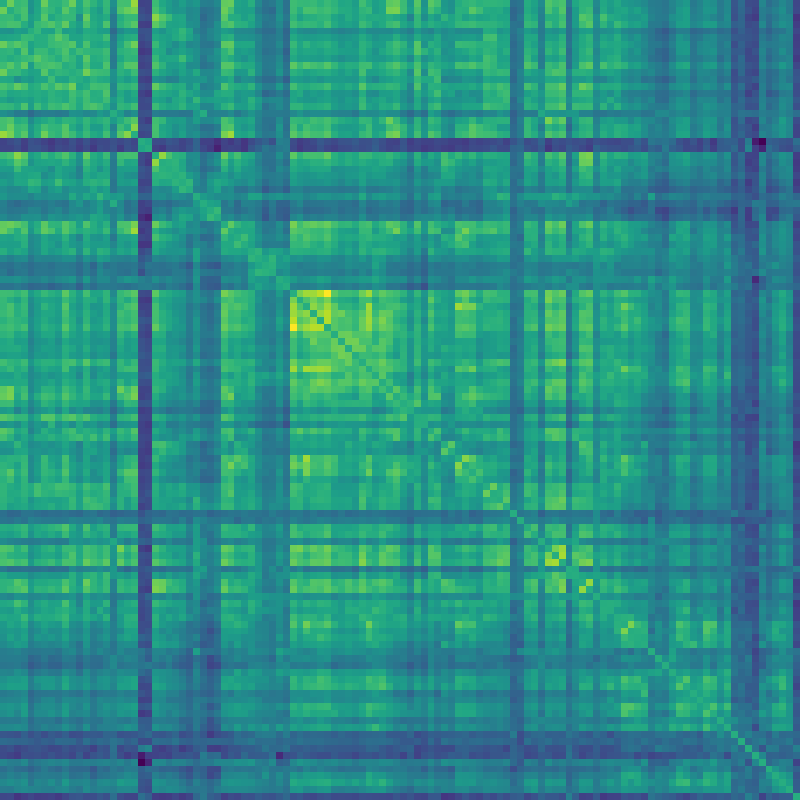
\includegraphics[width=\textwidth]{06_resultados_discusion/images/vae_recon_original_best.png}\\[3pt]
      {\small \textbf{FC original}}
    \end{column}
    \begin{column}{0.38\textwidth}
      \centering
      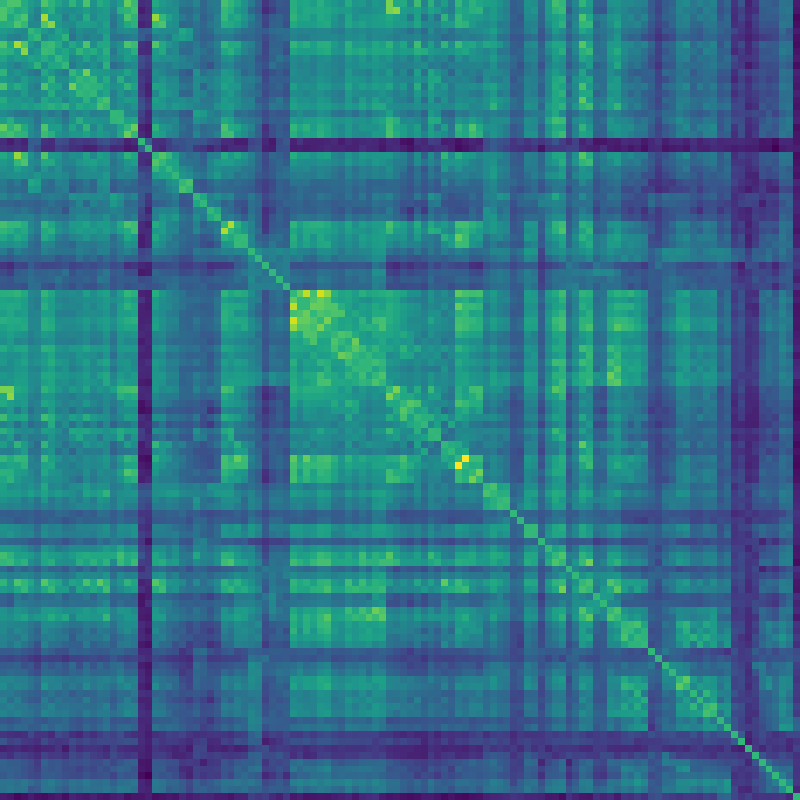
\includegraphics[width=\textwidth]{06_resultados_discusion/images/vae_recon_reconstructed_best.png}\\[3pt]
      {\small \textbf{FC reconstruida} ($r = 0{,}884$)}
    \end{column}
    \begin{column}{0.22\textwidth}
      {\scriptsize
      \begin{tabular}{lr}
        \toprule
        \textbf{Métrica} & \textbf{Val.} \\
        \midrule
        Pearson & 0,79 \\
        Coseno & 0,87 \\
        MAE & 0,124 \\
        \bottomrule
      \end{tabular}}

      \vspace{0.2cm}
      {\scriptsize \highlight{99\%} compresión\\$6670 \to 64$ dims}
    \end{column}
  \end{columns}

  \vspace{0.1cm}
  \centering
  {\small Patrones globales de conectividad preservados; detalles finos suavizados por la compresión.}
\end{frame}

\begin{frame}[shrink=3]{Resultado del modelo principal}{\color{uncyellow}\scriptsize $\blacktriangleright$ Objetivo 1: Predicción de edad cerebral}
  \begin{columns}[T]
    \begin{column}{0.48\textwidth}
      \centering
      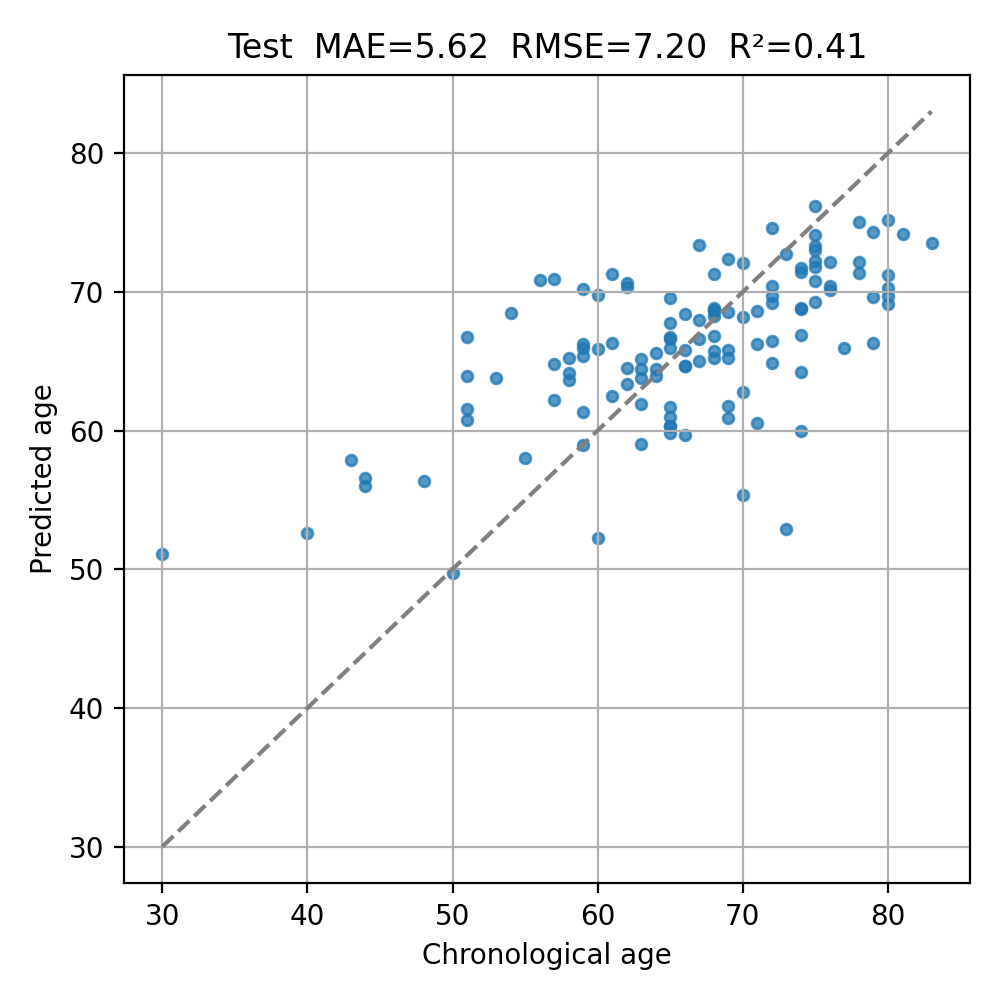
\includegraphics[width=0.88\textwidth]{06_resultados_discusion/images/xgb_scatter.png}\\[2pt]
      {\scriptsize Edad predicha vs.\ edad real ($n = 125$)}
    \end{column}
    \begin{column}{0.48\textwidth}
      \begin{block}{Métricas en test}
        \centering
        {\small
        \begin{tabular}{lr}
          \toprule
          \textbf{MAE} & \highlight{5,62 años} \\
          RMSE & 7,20 años \\
          $R^2$ & 0,411 \\
          Pearson & 0,644 \\
          \bottomrule
        \end{tabular}}
      \end{block}

      \vspace{0.05cm}
      {\small Error promedio de $\sim$5,6 años.\\Comparable con Gao et al.\ (5,92) con cohorte más diversa.}

      \vspace{0.05cm}
      {\scriptsize Mayor dispersión en extremos del rango etario.}
    \end{column}
  \end{columns}
\end{frame}

\begin{frame}{Importancia de features (XGBoost)}{\color{uncyellow}\scriptsize $\blacktriangleright$ Objetivo 1: Predicción de edad cerebral}
  \begin{columns}[T]
    \begin{column}{0.55\textwidth}
      \centering
      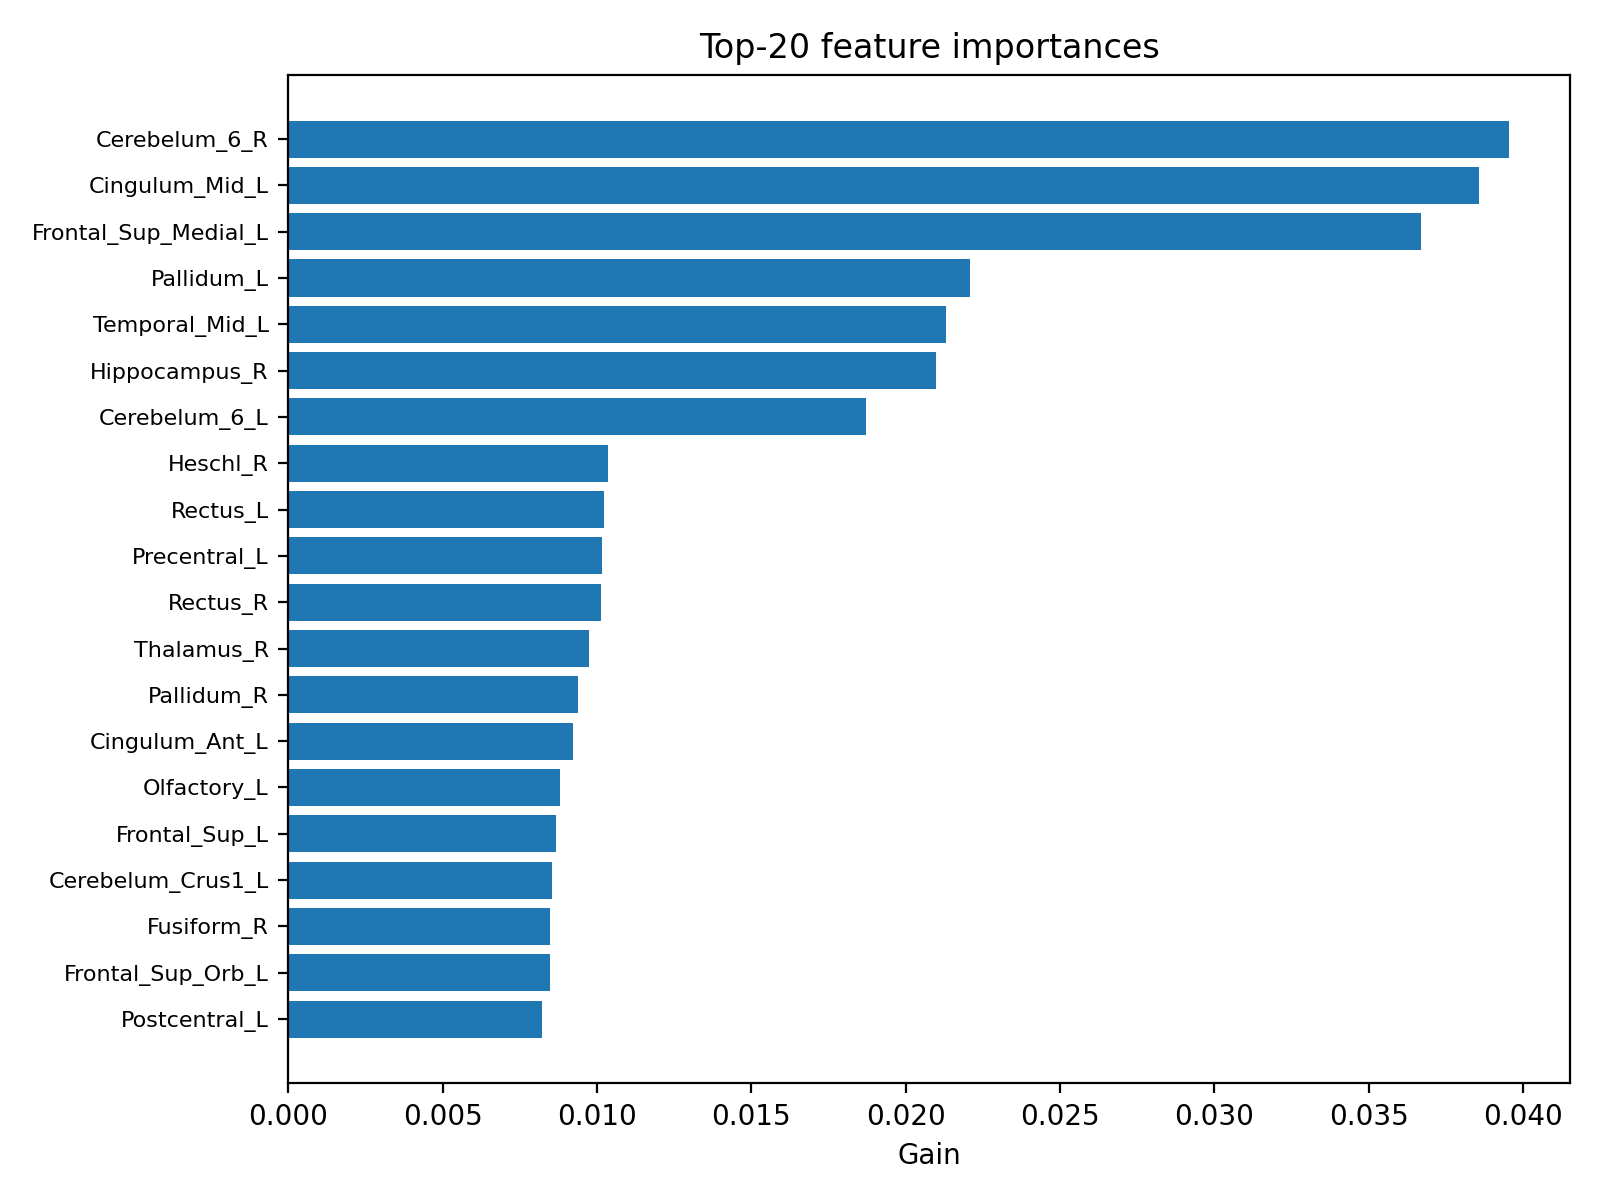
\includegraphics[width=\textwidth]{06_resultados_discusion/images/xgb_importance_top20.png}
    \end{column}
    \begin{column}{0.42\textwidth}
      {\small
      Las etiquetas son las regiones del atlas AAL (T1w) que más contribuyen a la predicción. Las que aparecen arriba (cerebelo, cíngulo, frontal, pallidum, temporal, hipocampo, tálamo) suelen reportarse en la literatura como estructuras con cambios asociados a la edad.

      \vspace{0.2cm}
      XGBoost da estas importancias de forma directa (Gain en los árboles). Con otros regresores, interpretar la contribución individual de cada feature resulta más complejo.
      }
    \end{column}
  \end{columns}
\end{frame}

\begin{frame}{Estudio de ablaciones}{\color{uncyellow}\scriptsize $\blacktriangleright$ Objetivo 1: Predicción de edad cerebral}
  \centering
  {\footnotesize
  \begin{tabular}{lrrrr}
    \toprule
    \textbf{Features} & \textbf{MAE} & \textbf{RMSE} & $\boldsymbol{R^2}$ & $\boldsymbol{r}$ \\
    \midrule
    Solo T1w (116) & 5,89 & 7,48 & 0,366 & 0,606 \\
    T1w + sexo (117) & 5,88 & 7,44 & 0,372 & 0,612 \\
    Solo $\beta$-VAE (64) & 7,01 & 9,12 & 0,056 & 0,284 \\
    $\beta$-VAE + sexo (65) & 7,06 & 9,18 & 0,044 & 0,268 \\
    \rowcolor{unclight}
    \textbf{$\beta$-VAE + T1w (180)} & \textbf{5,62} & \textbf{7,20} & \textbf{0,411} & \textbf{0,644} \\
    $\beta$-VAE + T1w + sexo (181) & 5,70 & 7,34 & 0,389 & 0,626 \\
    $\beta$-VAE + T1w + sexo + dx (182) & 5,64 & 7,17 & 0,416 & 0,648 \\
    \bottomrule
  \end{tabular}}

  \vspace{0.15cm}
  \begin{columns}[c]
    \begin{column}{0.48\textwidth}
      \begin{block}{Conclusiones}
        \begin{itemize}
          \item FC + T1w \highlight{$>$} cualquiera sola
          \item $\beta$-VAE solo: $R^2 = 0{,}056$ (insuficiente)
          \item Sexo y diagnóstico no mejoran
        \end{itemize}
      \end{block}
    \end{column}
    \begin{column}{0.48\textwidth}
      \centering
      \vspace{0.3cm}
      {\small Modalidades \highlight{complementarias}:\\
      agregar FC reduce MAE en 0,27 años\\respecto a T1w sola}
    \end{column}
  \end{columns}
\end{frame}

\begin{frame}{¿Importa cómo se comprime la conectividad?}{\color{uncyellow}\scriptsize $\blacktriangleright$ Objetivo 1: Predicción de edad cerebral}
  \begin{columns}[T]
    \begin{column}{0.48\textwidth}
      {\small \textbf{PCA vs.\ $\beta$-VAE} (misma dim.\ 64 + T1w):}

      \vspace{0.1cm}
      {\small
      \begin{tabular}{lrr}
        \toprule
        & \textbf{MAE} & $\boldsymbol{R^2}$ \\
        \midrule
        PCA + T1w & 5,61 & 0,431 \\
        $\beta$-VAE + T1w & 5,62 & 0,411 \\
        \bottomrule
      \end{tabular}}

      \vspace{0.15cm}
      {\small Rendimiento \highlight{prácticamente idéntico}.\\
      XGBoost captura no linealidades aun desde PCA.\\[4pt]
      {\scriptsize Optuna exploró solo 70 de un espacio vasto para el $\beta$-VAE.}}
    \end{column}
    \begin{column}{0.48\textwidth}
      {\small \textbf{FC crudo vs.\ comprimido:}}

      \vspace{0.1cm}
      {\small
      \begin{tabular}{lrrr}
        \toprule
        & \textbf{Feats} & \textbf{MAE} & $\boldsymbol{R^2}$ \\
        \midrule
        FC crudo + T1w & 6786 & 6,00 & 0,354 \\
        \rowcolor{unclight}
        \textbf{$\beta$-VAE + T1w} & \textbf{180} & \textbf{5,62} & \textbf{0,411} \\
        \bottomrule
      \end{tabular}}

      \vspace{0.15cm}
      {\small \highlight{97,3\%} menos features y mejor MAE.\\
      La \highlight{reducción} es lo clave,\\no si es lineal o no lineal.}
    \end{column}
  \end{columns}

  \objectivetracker{\objdone}{\objpend}{\objpend}
\end{frame}

\begin{frame}{Variables demográficas: educación}{\color{uncyellow}\scriptsize $\blacktriangleright$ Objetivo 2: Variables sociodemográficas}
  \begin{block}{Variable: \texttt{cog\_ed} --- años de educación formal (disponible 74,9\%)}
    {\small Indicador del nivel socioeconómico. Se analizó su correlación con la brain age gap por grupo diagnóstico.}
  \end{block}

  \vspace{0.2cm}
  \centering
  {\small
  \begin{tabular}{lrrl}
    \toprule
    \textbf{Grupo} & $\boldsymbol{r}$ & $\boldsymbol{p}$ & \textbf{Interpretación} \\
    \midrule
    CN  & $-0{,}067$ & $0{,}19$ & tendencia negativa, no significativa \\
    AD  & $+0{,}165$ & $0{,}002$ & significativa ($\uparrow$ educación $\rightarrow$ gap más alta) \\
    FTD & $\approx 0$ & $0{,}98$ & sin correlación \\
    \bottomrule
  \end{tabular}}

  \vspace{0.25cm}
  \begin{columns}[T]
    \begin{column}{0.46\textwidth}
      \begin{block}{CN}
        {\small Dirección negativa $\rightarrow$ educación como \textbf{factor neuroprotector} (reserva cognitiva). Señal débil con $n = 473$.}
      \end{block}
    \end{column}
    \begin{column}{0.46\textwidth}
      \begin{block}{AD}
        {\small Más educación $\rightarrow$ gap más positiva: diagnóstico tardío en estadios avanzados (\textbf{reserva cognitiva invierte el patrón}).}
      \end{block}
    \end{column}
  \end{columns}
\end{frame}

\begin{frame}{Variables demográficas: sitio y escáner}{\color{uncyellow}\scriptsize $\blacktriangleright$ Objetivo 2: Variables sociodemográficas}
  \begin{block}{El sitio de adquisición es el mayor confundidor}
    ANOVA: $F = 8{,}67$,\ $p < 0{,}001$ \quad $\rightarrow$ diferencias significativas entre los 11 centros.
  \end{block}

  \vspace{0.15cm}
  \begin{columns}[T]
    \begin{column}{0.52\textwidth}
      {\small
      \begin{tabular}{lrr}
        \toprule
        \textbf{Sitio} & $\boldsymbol{n}$ & \textbf{Gap media} \\
        \midrule
        Bruno       & 48  & $+4{,}30$ años \\
        Takada      & 89  & $+2{,}82$ \\
        Matallana   & 135 & $+0{,}92$ \\
        Miller      & 400 & $-0{,}20$ \\
        Lopera      & 88  & $-3{,}64$ \\
        \bottomrule
      \end{tabular}}
      \\[4pt]
      {\scriptsize Diferencia máxima $\approx$ 8 años entre sitios.}
    \end{column}
    \begin{column}{0.44\textwidth}
      \textbf{Por marca de escáner:}
      \vspace{0.1cm}
      {\small
      \begin{tabular}{lrr}
        \toprule
        \textbf{Escáner} & $\boldsymbol{n}$ & \textbf{Gap} \\
        \midrule
        Philips  &  47 & $+4{,}33$ \\
        GE       & 289 & $+0{,}95$ \\
        Siemens  & 581 & $-0{,}26$ \\
        \bottomrule
      \end{tabular}}
      \vspace{0.15cm}
      \begin{alertblock}{\small Conclusión}
        {\footnotesize El sitio explica la mayor parte de la varianza demográfica de la gap. Necesario: armonización \textbf{ComBat}.}
      \end{alertblock}
    \end{column}
  \end{columns}
\end{frame}

\begin{frame}{Demográficos como features: optimización con Optuna}{\color{uncyellow}\scriptsize $\blacktriangleright$ Objetivo 2: Variables sociodemográficas}
  \medskip
  {\small Se incluyen educación y sitio (\textit{one-hot}) como features adicionales. XGBoost optimizado con Optuna independiente por configuración.}

  \vspace{0.2cm}
  \centering
  {\small
  \begin{tabular}{lrrrr}
    \toprule
    \textbf{Configuración} & $\boldsymbol{n_{\text{test}}}$ & \textbf{MAE} & $\boldsymbol{R^2}$ & $\boldsymbol{r}$ \\
    \midrule
    $\beta$-VAE + T1w (baseline) & 125 & 5,62 & 0,411 & 0,644 \\
    + educación & 91 & 5,33 & 0,502 & 0,711 \\
    + sitio & 93 & 5,37 & 0,538 & 0,744 \\
    \rowcolor{unclight}
    \textbf{+ educación + sitio} & \textbf{91} & \highlight{5,17} & \textbf{0,523} & \textbf{0,725} \\
    \bottomrule
  \end{tabular}}

  \vspace{0.3cm}
  {\small MAE \highlight{5,17}: mejor configuración del trabajo. Mejora de \textbf{0,45 años} sobre el baseline.\\
  Las features demográficas aportan información \highlight{complementaria} a la neuroimagen; ambas aparecen en el top 20 de importancia.}

  \objectivetracker{\objdone}{\objdone}{\objpend}
\end{frame}

\begin{frame}{Entrenamiento solo en controles sanos}{\color{uncyellow}\scriptsize $\blacktriangleright$ Objetivo 3: Biomarcador de envejecimiento acelerado}
  \begin{block}{Idea}
    Entrenar solo con sujetos sanos ($n = 473$) y evaluar la brain age gap en \textbf{todos} los pacientes clínicos.
  \end{block}

  \vspace{0.15cm}
  \centering
  {\small
  \begin{tabular}{lrrrrr}
    \toprule
    \textbf{Grupo} & $\boldsymbol{n}$ & \textbf{MAE} & $\boldsymbol{R^2}$ & \textbf{Gap} \\
    \midrule
    CN (test)   & 53  & 6,03 & 0,504    & $-0{,}42$ \\
    AD (todos)  & 422 & 7,36 & $-0,170$ & $-1{,}86$ \\
    FTD (todos) & 297 & 6,93 & $-0,153$ & $+1{,}84$ \\
    \bottomrule
  \end{tabular}}

  \vspace{0.2cm}
  \begin{columns}[T]
    \begin{column}{0.46\textwidth}
      \begin{alertblock}{Problema}
        {\small MAE 6,03 en CN $>$ 5,62 (mixto)\\
        $R^2$ negativo en AD y FTD\\
        Gap inconsistente: $-1{,}86$ en AD}
      \end{alertblock}
    \end{column}
    \begin{column}{0.46\textwidth}
      \begin{block}{Conclusión}
        {\small Limitación es el \highlight{tamaño muestral}, no los hiperparámetros. Se necesitan $N > 2000$ CN.}
      \end{block}
    \end{column}
  \end{columns}
\end{frame}

\begin{frame}{CN-only + demográficos: hacia un biomarcador}{\color{uncyellow}\scriptsize $\blacktriangleright$ Objetivo 3: Biomarcador de envejecimiento acelerado}
  \begin{block}{Experimento exploratorio}
    {\small Entrenar solo con 337 CN (que tienen datos demográficos) incluyendo educación y sitio.}
  \end{block}

  \vspace{0.15cm}
  \centering
  {\small
  \begin{tabular}{llrrrr}
    \toprule
    \textbf{Modelo} & \textbf{Grupo} & $\boldsymbol{n}$ & \textbf{MAE} & \textbf{Gap} \\
    \midrule
    CN baseline (337) & CN (test) & 53 & 6,09 & $-0{,}07$ \\
                & AD       & 422 & 6,97 & $+0{,}21$ \\
                & FTD      & 297 & 7,42 & $+4{,}01$ \\
    \midrule
    CN + edu + sitio & CN (test) & 37 & \highlight{5,51} & $+0{,}41$ \\
                     & AD       & 348 & 6,41 & $+0{,}70$ \\
                     & FTD      & 211 & 6,49 & \highlight{$+4{,}11$} \\
    \bottomrule
  \end{tabular}}

  \vspace{0.2cm}
  {\small Gaps \highlight{consistentemente positivas} en AD y FTD $\rightarrow$ dirección esperada en neurodegeneración.\\
  Resultado prometedor: con más datos CN, el pipeline podría funcionar como biomarcador.}

  \objectivetracker{\objdone}{\objdone}{\objdone}
\end{frame}


\section{Discusión y conclusiones}

\begin{frame}{Discusión}
  \begin{itemize}
    \item \textbf{MAE de 5,62} dentro del rango de la literatura para cohortes comparables
    \begin{itemize}
      \item Gao et al.: MAE 5,92 con GNN ($N = 471$)
      \item Franke et al.: MAE 5,00 con RVM ($N = 650$, solo T1w)
    \end{itemize}

    \vspace{0.3cm}
    \item Trabajos con MAE $< 3$ usan cohortes \textbf{mucho mayores} ($N > 5000$)

    \vspace{0.3cm}
    \item La cohorte \highlight{latinoamericana} tiene mayor heterogeneidad (multi-sitio, multi-país)

    \vspace{0.3cm}
    \item $R^2 = 0{,}41$: queda varianza por explicar $\rightarrow$ margen de mejora

    \vspace{0.3cm}
    \item \highlight{CN-only + demográficos: MAE 5,51} --- mejor que el modelo mixto (5,62) y más comparable con la literatura (entrenan solo con sanos)
  \end{itemize}
\end{frame}

\begin{frame}{Limitaciones}
  \begin{enumerate}
    \item \textbf{Tamaño de la cohorte:} $N = 1245$ es modesto comparado con estudios recientes

    \vspace{0.25cm}
    \item \textbf{Heterogeneidad multi-sitio:} sin armonización entre centros (ComBat)

    \vspace{0.25cm}
    \item \textbf{Resolución del atlas:} AAL 116 regiones es grueso; atlas finos podrían capturar patrones más sutiles

    \vspace{0.25cm}
    \item \textbf{Sin modelos end-to-end:} no se comparó con 3D CNN ni GNN

    \vspace{0.25cm}
    \item \textbf{Exploración del $\beta$-VAE:} solo 70 trials de Optuna sobre un espacio combinatorio vasto; una mejor configuración podría superar a PCA
  \end{enumerate}
\end{frame}

\begin{frame}{Conclusiones}
  \begin{enumerate}
    \item Pipeline multimodal (FC + T1w) con MAE de \highlight{5,62 años}; con educación y sitio: \highlight{MAE 5,17}. CN-only + demográficos: \highlight{MAE 5,51}

    \vspace{0.18cm}
    \item La integración de ambas modalidades mejora la predicción\\$\rightarrow$ las fuentes son \highlight{complementarias}

    \vspace{0.18cm}
    \item $\beta$-VAE $\approx$ PCA con XGBoost optimizado; la \highlight{reducción} es clave: supera a FC crudo (5,62 vs.\ 6,00)

    \vspace{0.18cm}
    \item El \highlight{sitio de adquisición} es el mayor confundidor demográfico ($\sim$8 años de rango); armonización necesaria

    \vspace{0.18cm}
    \item CN-only + demográficos: \highlight{MAE 5,51} (mejor que mixto) con gaps positivas en AD y FTD $\rightarrow$ \highlight{prometedor} como biomarcador

    \vspace{0.18cm}
    \item Evaluado sobre cohorte \highlight{latinoamericana multicéntrica}; resultados relevantes en contexto LAC
  \end{enumerate}
\end{frame}

\begin{frame}{Trabajo futuro}
  \begin{columns}[T]
    \begin{column}{0.48\textwidth}
      \textbf{Datos:}
      \begin{itemize}
        \item Ampliar cohorte (especialmente CN, $N > 2000$)
        \item \textbf{Armonización multi-sitio} (ComBat, NeuroHarmonize)
        \item Atlas de mayor resolución
        \item Más features estructurales (materia blanca, LCR)
        \item Análisis demográfico ampliado (ingresos, ocupación, estatus socioeconómico y edad de inicio ---ao---)
      \end{itemize}
    \end{column}
    \begin{column}{0.48\textwidth}
      \textbf{Modelos:}
      \begin{itemize}
        \item Comparar optimización downstream vs.\ reconstrucción pura
        \item Modelos end-to-end (GNN, 3D CNN)
        \item Datos longitudinales
        \item Otras modalidades (DTI, grosor cortical)
      \end{itemize}
    \end{column}
  \end{columns}
\end{frame}


\begin{frame}{Agradecimientos}
  \vspace{2.5cm}
  \centering
  {\large Agradecimientos}
\end{frame}

\begin{frame}{}
  \vspace{2cm}
  \centering
  {\Huge \textcolor{uncblue}{¡Gracias!}}\\[1cm]
  {\Large ¿Preguntas?}\\[1.2cm]
  {\small
    Nicolás Marcelo Bazán\\
    FaMAF --- Universidad Nacional de Córdoba\\[0.35cm]
    Código: \url{https://github.com/BazanNicolas/Thesis-Computer-Science}
  }
\end{frame}

\end{document}
